\subsection{Объектно-ориентированная модель рекомендательной
системы}
Впервые объектно-ориентированная фильтрация была описана
Сарваром \cite{item-based} и Кариписом \cite{topn1,topn2}, а самой известной
ее практической реализацией является реализация
компании Amazon \cite{amazon-item2item}.

Коллаборативная фильтрация ООМ заключается в анализе характеристик
объектов, результатом которого является степень близости объектов.
Такой анализ производится с помощью мер близости $\di: I \times I \rightarrow
[0,1]$. Если степень близости объектов $i, j$ высока, то будем говорить, что
между этими объектами выполняется отношение близости $\rt$:
\begin{equation}
	\label{rt-ors}
\di(i, j) \ge \Delta_i \Leftrightarrow i \rt j,
\end{equation}
где $\Delta_i \in [0,1]$.
Объекты, между которыми выполняется отношение близости,
называются соседями \cite{item-based}.
В процессе решения объекты, между которыми не выполняется отношение близости,
отфильтровываются.

Данные модели используются, в основном, для решения задачи $topN$.

% ==============================================================================

\subsubsection{Задача $topN$}
Как говорилось во введении первой главы, правила вывода АКМ
основываются на эвристических утверждениях. Приведем эвристическое утверждение,
на котором базируется правило вывода $\Pi$ ООМ (далее это правило будем
обозначать $\Pi_O$), использующееся для решения
задачи $topN$ \cite{item-based,topn1,amazon-item2item}:
\begin{assert}\label{assertORS1}
Если пользователю нравится объект $i$, который
похож на объект $j$, то пользователю понравится объект $j$.
\end{assert}

Во введенной
терминологии данное утверждение примет следующий вид:
\begin{equation}
\label{ors-assert}
(u_a \R i) \wedge (i \rt j) \Rightarrow u_a \R j,
\end{equation}
где формально неопределенные термины, использующиеся в существующих
исследованиях, заменены на формальные обозначения.

На Рисунке \ref{amazon-ex1} приведен пример работы
сервиса LastFm, который иллюстрирует
работу РС при использовании правила вывода $\Pi_O$, основанного на утверждении
(\ref{assertORS1}): РС рекомендует пользователю музыкальных исполнителей,
между которыми и искомым выполняется отношение близости.

\begin{figure}[htb]
	\caption{Пример рекомендации сервиса LastFm. Искомый исполнитель ---
\textquotedblleft Pink Floyd \textquotedblright, снизу --- схожие исполнители}
\begin{center}
	\label{amazon-ex1}
 
\includegraphics[width=7in,height=7in]{pics/lstfm-rs-example.jpeg}
\end{center}
\end{figure}

В момент решения задачи $topN$ и в момент проверки качества решения
в ООМ используется информация только
о тех объектах, для которых известно, что $(u_a \R i_0) \wedge (u_a \R
i_{\bot})$\footnote{
	Во-первых, данная информация является достаточной для решения задачи
	$topN$, а, во-вторых, информация о других значениях $\rho(u, i)$
	может быть недоступна. К примеру, для случая интернет-магазина, где
	существует только факт наличия приобретения товара без его оценки.
	},
поэтому при решении задачи $topN$ будем работать с множеством исходных
данных вида $P = \{(u, i, \rho(u, i)): u \R i \}$.

Правило вывода $\Pi_O$ ООМ для решения задачи $topN$ задается следующей формулой:
\begin{equation}
	\label{ors-pi-top}
	i \rt i_0 \Rightarrow (\rh(u_a, i) := 1) \wedge (u_a \R i)
\end{equation}
Значения $\rh(u_a, i)$ задаются равными единице, потому что тогда объекты $i$
будут близкими для активного пользователя при любом пороговом значении
$\Delta_{\R}$.
Правило вывода $\Pi_O$ говорит о том,
что если существует объект $i$, являющийся соседом для объекта $i_0$,
то, следуя эвристическому утверждению модели (\ref{assertORS1}), выполняется
отношение $u_a \R i$,
так как $u_a \R i_0$ по принятому для задачи $topN$ виду исходного множества.
То есть решение можно записать в форме утверждения: $(u_a \R i_0) \wedge (i \rt
i_0) \Rightarrow u_a \R i$.

Приведем схему решения задачи $topN$ при использовании правила вывода $\Pi_O$
(\ref{ors-pi-top}). Для того, чтобы составить множество объектов, между которыми и
активным пользователем выполняется отношение близости, по правилу вывода нужно найти объекты,
между которыми и объектами обучающего множества будет выполняться отношение
близости. Тогда, следуя эвристическому утверждению, между найденными объектами
и активным пользователем будет выполняться отношение близости: пусть $i \rt
i_0$, тогда, так как по виду исходного множества, принятого для задачи $topN$
выполняется $u_a \R i_0$, по эвристическому утверждению (\ref{assertORS1})
выполняется $u_a \rt i$ ---
$(u_a \R i_0) \wedge
(i \rt i_0) \Rightarrow u_a \rt i$, --- что и требуется по задаче $topN$.

Схему решения задачи $topN$ можно описать как формирование кластера
объектов $\nit = \{ i : i \rt I^a_0 \}$,
$|\nit| = N$, где
$I^a_0 = \{i_0: \rho(u_a, i_0) \in P_0\}$ --- центр кластера. Множество
объектов кластера (кроме центра) является искомым решением.

Определим способы задания отношения близости между объектом $i$ и
подмножеством объектов $I^a_0$
\label{deltaTneighbours}
 \cite{topn1,topn2,amazon-item2item,disser0}:
\begin{itemize}
	\item $I^a_0 \rt i \Leftrightarrow \Bigr( \frac{1}{|I^a_0|} \cdot \sum \limits_{i_0
		\in I^a_0} \di(i,i_0) \Bigl) \ge \Delta_i$.
		В стандартном решении  \cite{item-based} $topN$
		для определения меры близости между объектом $i$ и множеством объектов
		$I^a_0$ вычисляется сумма мер близости между объектом $i$ и объектами
		$i_0 \in I^a_0$.
		$I^a_0 \rt i \Rightarrow \Bigr( \frac{1}{|I^a_0|} \cdot \sum \limits_{I^a_0 \in I^a_0}
		\di(i,I^a_0)\Bigl) \ge \Delta_i \Rightarrow \exists$
$i_0 \in I^a_0, I^a_0 \rt i$.
По данным задачи и вследствие выполнения отношения $I^a_0 \rt i$, выполняется
		$(u_a \R I^a_0) \wedge (I^a_0 \R i) \Rightarrow u_a \R i$. Таким образом,
если объект $i$ принадлежит кластеру $\nit$ (то есть выполняется
		$I^a_0 \rt i$), то по утверждению ООМ  (\ref{assertORS1}) выполнится $u_a \R i$.
Поэтому данный способ определения отношения $i \rt I^a_0$ можно
		применять с правилом вывода $\Pi_O$ (\ref{ors-pi-top}) для решения задачи

\item $I^a_0 \rt i \Leftrightarrow$  $\exists I^a_0 \in I^a_0, I^a_0 \rt i$.
По данным задачи и способу задания $I^a_0 \rt i$ выполняется утверждение ООМ, то есть
		$(u_a \R I^a_0) \wedge (I^a_0 \rt i) \Rightarrow u_a \R i$.

Таким образом, если объект $i$ принадлежит кластеру $\nit$ (то есть $I^a_0 \rt i$),
		то по утверждению ООМ (\ref{assertORS1}) выполнится $u_a \R i$, что и требуется
от задачи.
Поэтому данный способ определения отношения $i \rt I^a_0$ можно
		применять с правилом вывода $\Pi_O$ (\ref{ors-pi-top}) для решения задачи
$topN$.
\end{itemize}
%%% Для вычисления значения меры близости между объектами системы может использоваться самая различная информация об объектах, которая
%%% зависит от реализации и предметной области РС\footnote{Поэтому при описании схемы, как 
%%% правило, не уделяется внимание контентам объектов}. К примеру, для кинематографической РС сценарий рекомендаций можно описать так: 
%%% если пользователь приобрел коллекцию DVD <<Крестный отец>>, то система может произвести рекомендации тех DVD, 
%%% где участвует Марлон Брандо, режиссером которых является Френсис Форд Коппола, или в жанре криминальная драма. 
%%% То есть характеристиками объекта может выступать любая
%%% известная и значительная информация о нем, в данном случае это: известный актер, режиссер и жанр.
%%--------------------------------------------
\bigbreak
Опишем один из вариантов исполнения ООМ и решим
задачу $topN$  \cite{item-based}.%TODO: set cite
\begin{itemize}
	\item $c_X(u_a) = (x_1, x_2, ..., x_|I|)$
		\begin{equation*}
			x_i =
			\begin{cases}
				1, &\text{если $u_a \R i$}\\
				0, &\text{иначе}
			\end{cases}
		\end{equation*}
		контент активного пользователя --- вектор {\it бинарных} оценок,
		отображающий информацию о том, какие объекты пользователь предпочитает.
		Примером такого контента является контент пользователя
		РС Amazon \cite{amazon-item2item}, где $x_i = 1$ означает то, что пользователь
		приобрел товар $i$;
	\item контент объекта в исследованиях РС, как правило,
		не определяется, так как множество характеристик объектов,
		их значений и структура контента не влияют на технику решения и могут
		варьироваться для различных реализаций РС. В описываемой модели
		воспользуемся векторным представлением, то есть
		$c_Y = (y_1,...,y_{|Y|})$;
	\item
		$\di(i,j) =\cos(\angle(c_Y(i),c_Y(j)))$.

		Типичной мерой близости, используемой при решении задачи $topN$ является
		косинус угла между контентами объектов, представляемых в виде векторов
		\cite{item-based,rs-handbook}.
	\item
		Чтобы не производить расчеты меры близости при формировании
		$\overline{P}^a_{\bot}$ каждый раз, когда активный пользователь
		делает запрос на решение задачи $topN$, значения мер близости $\di$
		рассчитываются заранее и заносятся в специальную матрицу $\mathbb{M}$
		размера $|I| \times |I|$:
		\begin{equation*}
			\mathbb{M}_{ij} =
			\begin{cases}
				\di(i,j), & i \ne j \\
				0, & \text{иначе}
			\end{cases}
		\end{equation*}

		Такой предварительный этап называется построением модели \cite{topn2}.
\end{itemize}

На рисунке (\ref{dia:matrix}) изображена блок-схема алгоритма
построения матрицы $\mathcal{M}$, которой соответствует псевдокод, представленный на изображении <<Алгоритм построения матрицы мер близости объектов>>  (\ref{alg:matrix})
\begin{figure}[htb]
	\caption{Блок-схема алгоритма построения матрицы $\mathcal{M}$}
\begin{center}
	\label{dia:matrix}
 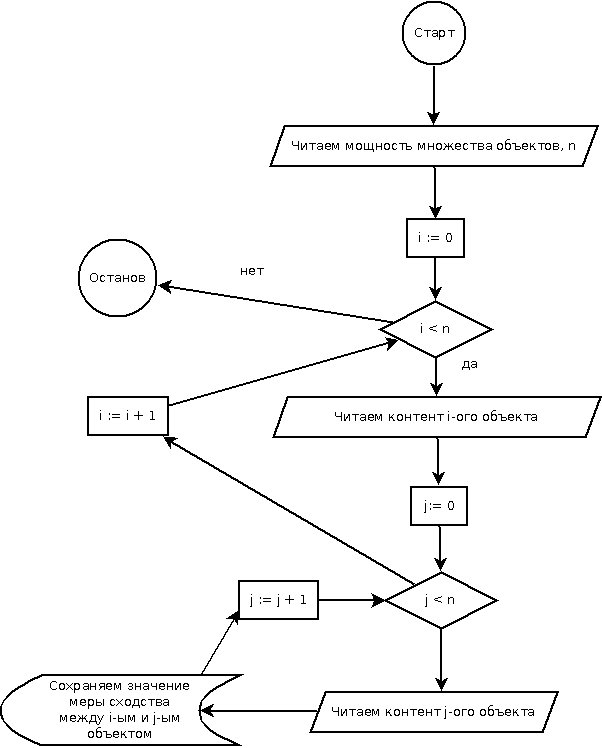
\includegraphics[width=6in,height=7in]{pics/algs/matrix.png}
\end{center}
\end{figure}

%\begin{figure}[htbp]
\begin{figure}[htb]
\caption{Алгоритм построения матрицы мер близости объектов}
\label{alg:matrix}
%\begin{algorithm}
\begin{algorithmic}[1]
\For{$i \gets 1, i \le n$}
	\State $\mathbb{M}_{ii} \gets 0$ \Comment{Чтобы пара с одинаковыми
	объектами не участвовала в дальнейших расчетах}
  \For{$j \gets 1, j \le n$}
  \State $\mathbb{M}_{ij} \gets \di(i,j)$
  \State $\mathbb{M}_{ji} \gets \mathbb{M}_{ij}$
  \State $j \gets j + 1$
  \EndFor
\State $i \gets i + 1$
\EndFor
\end{algorithmic}
%\end{algorithm}
\end{figure}

Для нахождения решения задачи $topN$ построим вектор
$\mathit{M} = (\overline{x}_1,...,\overline{x}_|I|)$, где
$
\overline{x}_i =
\begin{cases}
	0, &\text{если  $i \in I^a_0 $}\\
\mathbb{M}^i \times c_X(u_a)^T, &\text{ иначе }
\end{cases}
$\\
$c_X(u_a)^T$ --- транспонированный контент-вектор активного пользователя.
$I_{topN} = \{ i \in \{\overline{x}_i\} )\}$, где
$\{\overline{x}_i\}$ --- множество, состоящее из $N$ наибольших значений
координат вектора $\mathit{M}$.

На рисунке <<Блок-схема стандартного алгоритма решения задачи $topN$ в ООМ>> (\ref{dia:topn-solve-ors}) изображена блок-схема стандартного
алгоритма алгоритма решения задачи $topN$ в ООМ, которой соответствует
псевдокод, представленный на изображении <<Стандартный метод решения задачи $topN$ в ООМ>> (\ref{alg:topn-solve-ors})
\begin{figure}[htb]
	\caption{Блок-схема стандартного алгоритма решения задачи $topN$ в ООМ}
\begin{center}
	\label{dia:topn-solve-ors}
 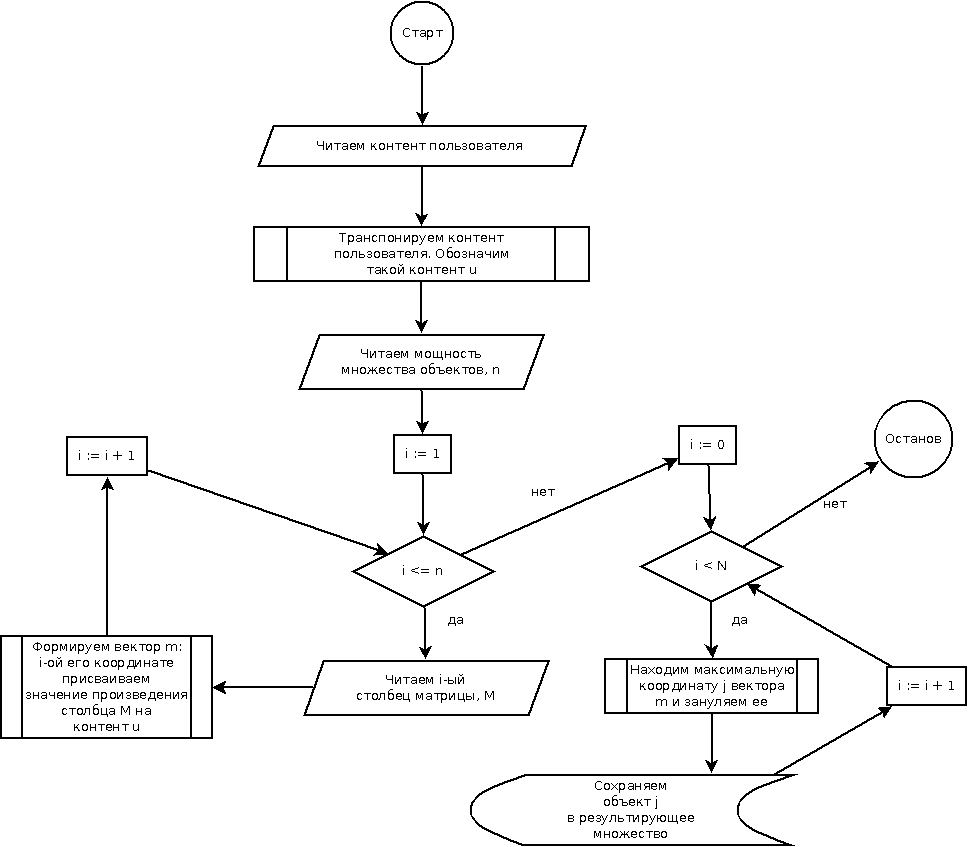
\includegraphics[width=7in,height=8in]{pics/algs/topn-ors.png}
\end{center}
\end{figure}

\begin{figure}[htb]
%\begin{algorithm}
\caption{Стандартный метод решения задачи $topN$ в ООМ}
\label{alg:topn-solve-ors}
\begin{algorithmic}[1]
\For{$i \gets 1, l \le n$} \Comment{Умножаем вектор-контент на матрицу}
	\State $m_i \gets \mathbb{M}^i \times c_X(u_a)^T$
\EndFor
\For{$j \gets 1, j \le N$}
	\State $i \gets \underset{i}{\mathrm{argmax}} \text{ } \overline{x}_i$
	\State $I_{topN} \gets I_{topN} \bigcup \{i\}$
	\Comment{Выбираем координату вектора $\mathit{M}$ с наибольшим значением}
\bigbreak
  \State $\overline{x}_i \gets 0$ \Comment{Зануляем уже выбранную координату}
  \State $j \gets j + 1$
\EndFor
\end{algorithmic}
%\end{algorithm}
\end{figure}


\subsubsection{Задача прогнозирования}
Эвристическое утверждение, на котором основывается решение задачи
$pred$ в ООМ, является более общим случаем утверждения
(\ref{assertORS1}):
\begin{assert}
	\label{assertORS2}
	Если два объекта схожи, то заданные им оценки близости пользователя будут
	приблизительно равны. \cite{rs-handbook,melville}.
\end{assert}
Данное утверждение является более общим случаем утверждения ООМ
(\ref{assertORS1}),
которое
используется при решении задачи $topN$,
так как рассматривает любые оценки, поставленные пользователем,
а не только те, которые означают, что между пользователем и объектом
выполняется отношение близости.

Во введенной терминологии данное утверждение примет следующий вид:
\begin{equation}
	i \rt j \Leftrightarrow |\rho(u,i) - \rho(u,j)|
	\le \varepsilon_p
\end{equation}

Правило вывода ООМ для решения задачи $pred$ запишется следующей
формулой:
\begin{equation}
	\label{ors-pi-p}
	\rh(u_a, i_{\bot}) = g_p(\{\rho(u_a, i^{\prime}_0)\}),
	i^{\prime}_0 \rt i_{\bot}.
\end{equation}
Правило вывода говорит о том, что оценки близости между
пользователем $u_a$ и объектами, являющимися соседями,
функционально связаны. Таким образом, зная
оценки близости, которые пользователь уже задал объектам
$i \rt i_{\bot}$, можно вычислить $\rh(u_a, i_{\bot})$
на основании функциональной связи
$g_p$.

Схема решения задачи $pred$ заключается в построении кластера
$\nip = \{ i_0 : i_0 \rt i_{\bot}\}$, центром которого является прогнозируемый
объект $i_{\bot}$. Решение задачи $pred$ запишется в виде:
\begin{equation}\label{pred-f}
	\rh(u_a,i_{\bot}) = g_p(\{\rho(u_a, i_0): i_0 \in \nip \}
\end{equation}
где $g_p$ --- некоторая функция, используемая в модели для
формирования по множеству оценок пользователя прогнозной оценки.

%===================================================================
%--------------------------------------------
%===================================================================
Опишем возможную\footnote{Модели могут отличаться такими параметрами, как,
например, функция $\di$, поэтому нижеописанная модель является одной из
возможных}
реализацию ООМ
\footnote{
	На данном этапе без оценки качества $\mathcal{E}_{topN}$
	}
 и на ее примере решим
задачу прогнозирования  \cite{item-based} %TODO: set cite. I think need
												%to see amazon
\begin{itemize}
	\item $c_X(u_a) = \{\rho(u_a,i_0)\}$
	\item $c_Y = (y_1,...,y_{|Y|})$;
	\item $\di(i,j) = \cos(\angle(c_Y(i),c_Y(j)))$
\end{itemize}
\bigbreak

Прогнозирование строится на основании оценок, поставленных активным пользователем
объектам, между которыми и прогнозируемым выполняется отношение близости.
Поиск таких объектов может осуществляться линейно по значениям, которые уже
хранятся в матрице мер близости $\mathbb{M}$, находящихся в строке с порядковым
номером, соответствующим индексу объекту. После построения кластера соседей
$\nip$,
вычисляется значение {\it прогнозной функции} от оценок пользователей,
поставленных $i \in \nip$.


На рисунке (\ref{dia:p-ors}) изображена блок-схема алгоритма
решения задачи $pred$ в ООМ.
\begin{figure}[htb]
	\caption{Блок-схема алгоритма построения матрицы $\mathcal{M}$}
\begin{center}
	\label{dia:p-ors}
 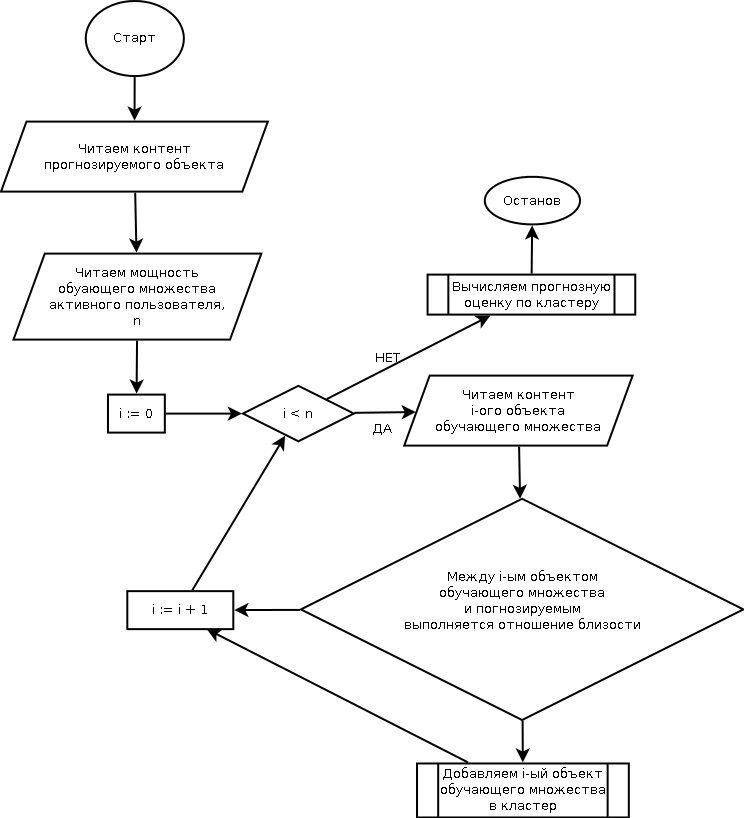
\includegraphics[width=7in,height=8in]{pics/algs/p-ors.png}
\end{center}
\end{figure}
Блок-схеме алгоритма решения задачи $pred$ в ООМ соответствует
псевдокод, представленный на изображении <<Стандартный алгоритм решения задачи $pred$ в ООМ>>  (\ref{alg:p-ors}).

\begin{figure}[htb]
\caption{Стандартный алгоритм решения задачи $pred$ в ООМ}
\label{alg:p-ors}
	%\begin{algorithm}
\begin{algorithmic}[1]
\State $\nip \gets \varnothing$\Comment{Множество объектов,
	оцененных активным пользователем и схожих с прогнозируемым объектом}
	\State $l \gets i_{\bot}$\Comment{Сохраняем в переменной $l$ индекс
	прогнозируемого объекта}
	\State $P^a \gets \varnothing$ \Comment{Множество оценок близости
	активного пользователя}
	\For {$i \in I^a_0$}
	\If {$\mathbb{M}^i_l \ge \Delta_i$}\Comment{Объект $i$ близок к
	прогнозируемому}
  \State $\nip \gets \nip \bigcup \{ i \}$
	\State $P^a \gets P^a \bigcup \{\rho(u_a,i)\}$
  \EndIf
\EndFor
\State $\rh(u_a,i) \gets g_p( P^a )$\Comment{Рассчитываем значение функции прогнозирования}
\end{algorithmic}
%\end{algorithm}
\end{figure}


\subsubsection{Функции вычисления прогнозной оценки}
Приведем
пример распространенной функции прогнозирования, применяемой в ООМ
 \cite{item-based}:
%cite
\begin{equation}\label{fpredict-ors}
	\frac{1}{|\nip|} \frac{\sum \limits_{i \in \nip} \di(i,i_{\bot}) \cdot \rho(u_a,i)}{
\sum \limits_{i \in \nip} \di(i,i_{\bot})
}
\end{equation}
%===================================================================
%--------------------------------------------
%===================================================================
\subsubsection{Используемые функции в качестве меры сходства}
\begin{itemize}
% ToDo: information retireval bib
\item \textbf{Косинус.} \newline
Наиболее популярная мера сходства, заимствованная из области
информационного поиска \cite{ir1,ir2,ir3}:
\begin{equation} \label{sim-cos}
	cos(\angle(c_Y(i),c_Y(j)) = \frac{\sum \limits_{k=1}^{|Y|} y^i_k \cdot y^j_k}{
		\sqrt{ \sum \limits_{k=1}^{|Y|} (y^i_k)^2 } \cdot
		\sqrt{ \sum \limits_{k=1}^{|Y|} (y^j_k)^2 }},
\end{equation}

\item {\bf Условная вероятность.} \newline
Данная мера сходства была разработана Кариписом \cite{topn1} для такой
предметной области РС, в которой оценки близости принадлежат бинарной
шкале. Оценки близости обладают семантикой условной вероятности
события (к примеру, приобретения товара),
которое зависит от истории поведения пользователя:
$Pr( \rho(u_a,i) = 1 | \rho(u_a,j) = 1 )$
\begin{equation}
Pr(i,j) = \frac{\tf(i \wedge j)}{\tf(i) \cdot \tf(j)^{\alpha}}
\end{equation}
где:
\begin{itemize}

\item $\tf(i)$ --- весовой коэффициент, использование которого заимствовано из
области информационного поиска, этот коэффициент определяет частоту
(от term frequency), с какой объект оценивается пользователями, то есть
$\tf(i) = |\{\rho(u,i): \rho(u,i) \in P_0\}|$,
$\tf(i ^ j) = |U^i \bigcup U^j|$,
$U^i = \{u: \rho(u_a,i) \in P_0\}$,
$U^j = \{u: \rho(u,j) \in P_0\}$.

\item $\alpha$ --- коэффициент, который служит для учета популярных объектов,
имеющих, к примеру, тенденцию быть приобретенными большинством пользователей
(и иметь, таким образом, большое значение частоты).

\end{itemize}

\item {\bf Коэффициент корреляции Пирсона.} Мера сходства,
заимствованная из статистики. Данная мера сходства использовалась
компаниями GroupLens \cite{grouplens} и Bellcore \cite{bellcore}.
\begin{equation}
 \frac{\sum \limits_{y}(y^1 - \overline{y^1}) \cdot (y^2 -
                                           \overline{y^2})}
                {\sqrt{\sum \limits_{y}(y^1 - \overline{y^1})^2 \cdot
        \sum \limits_{y}(y^2 - \overline{y^2})^2}},
\end{equation}

$\overline{y^k}$ -- среднее значение характеристики $k$-ого объекта.
\end{itemize}


\subsubsection{Примеры решения задач}
Рассмотрим примеры решения задач помощью ООМ.
\paragraph{Данные}
\begin{itemize}
\item
	Пусть контенты объектов некоторой системы представляют
		собой вектора в трехмерном пространстве характеристик $Y =
		\{y_1,y_2,y_3\}$, значения характеристик
	--- действительные числа.
	Пусть в системе существуют объекты со следующими контентами:
  \begin{enumerate}
  \item $c_Y(1) = (0,2; 0,8; 0)$;
  \item $c_Y(2) = (0; 1; 0)$;
  \item $c_Y(3) = (0,2; 1; 0)$;
  \item $c_Y(4) = (0; 0,2; 0)$;
  \item $c_Y(5) = (1; 0; 0)$;
  \item $c_Y(6) = (0,8; 0; 0)$;
  \item $c_Y(7) = (0; 0; 1)$;
  \item $c_Y(8) = (0; 0; 0,8)$;
  \item $c_Y(9) = (0; 0; 1)$;
  \end{enumerate}
\item Матрица мер сходства:\\
$\mathbb{M} = $
$
\begin{pmatrix}
0    & 0.97 & 0.99   & 0.97 & 0.24 & 0.19 & 0 & 0    & 0    \\
0.97 & 0    & 0.98   & 1    &   0  &  0   & 0 & 0    & 0    \\
0.99 & 0.98 & 0      & 0.97 & 0.58 & 0.19 & 0 & 0    & 0    \\
0.97 & 1    & 0.97   & 0    & 0.37 & 0    & 0 & 0    & 0    \\
0.24 & 0    & 0.58   & 0.37 & 0    & 1    & 0 & 0    & 0    \\
0.19 & 0    & 0.19   & 0    & 1    & 0    & 0 & 0    & 0    \\
0    & 0    & 0      & 0    & 0    & 0    & 0 & 0.98 & 1    \\
0    & 0    & 0      & 0    & 0    & 0    & 0.98 & 0 & 0.98    \\
0    & 0    & 0      & 0    & 0    & 0    & 1    & 0.98 & 0    \\
\end{pmatrix}
$
\item $c_X(u_a) = (1;1,0,0,0,0,1,0,0)$
\item $N = 2$ --- для задачи $topN$ нужно определить
	два объекта, между которыми и активным пользователем выполняется отношение
		близости;
\end{itemize}

\paragraph{Решение задачи $topN$}
\begin{enumerate}
\item В матрице $\mathcal{M}$ в каждом столбце оставляем $N$
	наибольших элементов:
$\mathcal{M'} = $
$
\begin{pmatrix}
0    & 0,97 & 0,99   & 0,97 &      & 0,19 & 0 & 0    & 0    \\
0,97 & 0    & 0,98   & 1    &   0  &  0   & 0 & 0    & 0    \\
0,99 & 0,98 & 0      &      & 0,58 & 0    & 0 & 0    & 0    \\
0    & 1    & 0      & 0    &      & 0    & 0 & 0    & 0    \\
0    & 0    & 0      & 0    & 0    & 1    & 0 & 0    & 0    \\
0    & 0    & 0      & 0    & 1    & 0    & 0 & 0    & 0    \\
0    & 0    & 0      & 0    & 0    & 0    & 0 & 0,98 & 1    \\
0    & 0    & 0      & 0    & 0    & 0    & 0,98 & 0 & 0,98    \\
0    & 0    & 0      & 0    & 0    & 0    & 1    & 0,98 & 0    \\
\end{pmatrix}
$
\item Перемножим {\it транспонированный} контент $c_X(u_a)^T$
	пользователя и матрицу $\mathcal{M'}$
		$m = (u_a)^T \times \mathcal{M'} = s = (0,97; 0,97, 1.97, 1.97, 0, 0,19, 0, 0,98, 1)$
\item Из вектора $m$ выбираем два наибольших значения. Им
	соответствуют объекты 3 и 4. Поэтому
		$I_{topN} = \{3, 4\}$.
\end{enumerate}

\paragraph{Задача прогнозирования}
Решим задачу прогнозирования для объекта 4 и активного пользователя со
следующими данными $P^a_0 = \{(2 | 1), (3, 0,1)\}$.
\begin{enumerate}
	\item $i_{\bot} = 4$ --- необходимо спрогнозировать оценку 4-ого объекта;
	\item Будем пользоваться функцией прогнозирования, описанной формулой
		(\ref{pred-f}).
	\item Составим множество соседей прогнозируемого объекта 4, для чего
		воспользуемся матрицей $\mathcal{M}$, $\nip = \{2, 3\}$
\item $\rho(u_a, 4) = \frac{1 \cdot 0.97 + 0,9 \cdot 1}{|0.97 + 1|} = 0,95$
\end{enumerate}

%===================================================================
%--------------------------------------------
%===================================================================
%===================================================================
%--------------------------------------------
%===================================================================

%-----------------------------------------------
%% \subsubsection{Примеры решения задач ООМ}
%% Рассмотрим примеры решения задач в ООМ. Будем использовать в примерах одни и те же данные
%% для каждой задачи, которые были описаны в разделе 1.3.6.

%% \paragraph{Задача top-$N$}
%% Решим задачу top-$N$ при $N=2$. Известно, что 
%% $I^a = \{ (i^1; 0,9), (i^2; 0,75), (i^5; 0,5), (i^6; 0,3), (i^{10}; 0,8)  \}$, поэтому контент активного пользователя
%% при решении задачи top-$N$ представляется в виде следующего вектора:
%% $a =
%% \begin{pmatrix} 
%% 1\\
%% 1\\
%% 0\\
%% 0\\.Ь = 
%% 0\\
%% 0\\
%% 0\\
%% 0\\
%% 0\\
%% 1\\
%% \end{pmatrix}
%% $
%% \begin{enumerate}
%% \item Предварительно проведем этап моделирование, в ходе которого построим матрицу оценок сходства $\mathbb{M}$
%% $
%% \begin{pmatrix} 
%% 0    & 0,99 & 0,76 & 0,47 & 0,62 & 0,07 & 0,98 & 0    & 0,26 & 0,7  \\
%% 0,99 &  0   & 0,74 & 0,5  & 0,69 & 0,14 & 0,96 & 0,08 & 0,35 & 0,74    \\
%% 0,76 & 0,74 & 0    & 0,8  & 0,39 & 0,31 & 0,85 & 0,21 & 0,24 & 0,1   \\
%% 0,47 & 0,5  & 0,8  & 0    & 0,63 & 0,81 & 0,55 & 0,74 & 0,69 &   0  \\
%% 0,62 & 0,69 & 0,39 & 0,63 & 0    & 0,71 & 0,54 & 0,7  & 0,91 & 0,91   \\
%% 0,07 & 0,14 & 0,31 & 0,81 & 0,71 & 0    & 0,08 & 0,99 & 0,92 & 0  \\
%% 0,98 & 0,96 & 0,85 & 0,55 & 0,54 & 0,08 & 0    &  0   & 0,21 &   0,57 \\
%% 0    & 0,08 & 0,21 & 0,74 & 0,7  & 0,99 & 0    &  0   & 0,92 &  0  \\
%% 0,26 & 0,35 & 0,24 & 0,69 & 0,91 & 0,92 & 0,21 & 0,92 & 0    & 0,37   \\
%% 0,7  & 0,74 & 0,1  & 0    & 0,91 & 0    & 0,57 &  0   & 0,37 & 0    \\
%% \end{pmatrix}
%% $

%% \item В полученной матрице в каждом столбце оставляем $N (=2)$ наибольших элементов:
%% $\mathcal{M'} = \\$
%% $
%% \begin{pmatrix} 

%% \end{pmatrix}
%% $
%% \item Перемножим {\it транспонированный} вектор-контент пользователя и матрицу, полученную в пункте 4:
%% $(u_a)^T \bot \mathcal{M'} = s = (0.97, 0.97, 1.97, 1.97, 0, 0.19, 0, 0.98, 1) \Rightarrow I^a_{topN} = \{i^3, i^4\}$
%% \end{enumerate}
%% \paragraph{Задача прогнозирования}
%% \begin{enumerate}
%% \item Из вида матрицы и условия\ref{example-cond}  следует, что что $\{i^1,i^2,i^3\}$ --- множество объектов, схожих с прогнозируемым;
%% \item $\rho(u_a, i^4) = \frac{1 \cdot 0.97 + 0.9 \cdot 1}{|0.97 + 1|} = 0.95$
%% \item Результат прогнозирования соответствует результату задачи top-$N$, так как $vp^a_l = 9.5 \Rightarrow a \R i$, и $i \in I^a_{topN}$
%% \end{enumerate}



%% \subparagraph{Характеристика объектно-ориентированных систем}
%% \subsubparagraph{Асимптотическая сложность решения и модели}
%% Для построения матрицы мер сходства необходимо вычислить $\frac{1}{2} \cdot (|T| - 1) \cdot |T|$ раз меру сходства. Сложность вычисления меры 
%% сходства зависит от мощности $C_T$. Однако $|CT| << |T|$, поэтому будем считать, что сложность вычисления меры сходства -- константа,
%% а {\bf асимптотическая сложность} определяется формулой $O(|T|^2)$.
%% {\bf  асимптотическая сложность} решения определяется умножением матрицы на вектор, она равна $O(|T|^2)$.

%% % ToDo сослаться на Сашину систему
%% Сложность данного решения велика, учитывая тот факт, что, как правило, в реальных систем $T$ огоромно. К примеру, 
%% новостная лента каждый день пополняет свою базу более, чем на 100 статей объектов. Таким образом, модель и решение
%% ООМ обладает {\it слабой масштабируемостью}.
%


%-----------------------------------------------

